\documentclass[dvips]{beamer}
% [dvips] allows use of latex->dvips->ps2pdf instead of pdflatex

\usepackage{beamerthemesplit}
\usepackage{amsmath,amssymb,amsfonts,amsthm}
%\usepackage{graphicx,psfrag} %only include if using pictures with psfrag
\usepackage[T1]{fontenc} 
%\usepackage{figures/subfig}
\usepackage{subfigure}
\let\Tiny=\tiny


\mode<presentation>
{
  %\usetheme{Berkeley}   % left bar
  %\usetheme{Antibes} % tree header
  %\usetheme{Boadilla}  % very plain
  %\usetheme{Warsaw}
  %\usetheme{Rochester} %
  %%\usetheme{Goettingen}  % right bar
  %\usetheme{Ilmenau}

  %\usepackage{beamerouterthemeshadow}
  %\usepackage{beamerouterthemesmoothtree}
  %\usepackage{beamercolorthemeorchid}
  %\usepackage{beamerinnerthemerounded}

  %\setbeamercovered{transparent}
  % comment out to completely hide covered material
}

% **** All themes: remove comment and find out which one you like!

%\usetheme{Warsaw}
\usetheme{Frankfurt} % I like it.
%\usetheme{Szeged}
%\usetheme{Singapore}
%\usetheme{Rochester}  % no menus at top
%\usetheme{Pittsburgh}
%\usetheme{Berlin}   % too much header/footer stuff
%\usetheme{Antibes}
%\usetheme{Bergen} % very large side margins
%\usetheme{Boadilla} % nice and simple
%\usetheme{boxes}
%\usetheme{Copenhagen}
%\usetheme{Darmstadt}
%\usetheme{default}
%\usetheme{Dresden}
%\usetheme{Goettingen}
%\usetheme{Hannover}
%\usetheme{Ilmenau}
%\usetheme{JuanLesPins}
%\usetheme{Luebeck}
%\usetheme{Madrid}
%\usetheme{Malmoe}
%\usetheme{Marburg}
%\usetheme{Montpellier}
%\usetheme{PaloAlto}

%You can also pick a color theme in addition to theme above.

%\usecolortheme{albatross}
%\usecolortheme{beetle}
%\usecolortheme{crane}
%\usecolortheme{dolphin}
%\usecolortheme{dove}
%\usecolortheme{fly}
%\usecolortheme{lily}
%\usecolortheme{seagull}
%\usecolortheme{seahorse}
%\usecolortheme{rose}


%\usefonttheme[onlylarge]{structuresmallcapsserif}


%\usepackage{times}
%\usepackage[T1]{fontenc}
% Or whatever. Note that the encoding and the font should match. If T1
% does not look nice, try deleting the line with the fontenc.


\newtheorem{thm}{Theorem}




% ************************ space ************************************
\newcommand{\hhs}[1]{\hspace{#1mm}}
\newcommand{\hs}{\hspace{5mm}}
\newcommand{\vp}{\vspace{1mm}}
\newcommand{\vs}{\vspace{5mm}}
\newcommand{\jl}{$\frac{}{}$} %User defined for empty symbol to jump line
% ********************** newcommand *********************************
\newcommand{\mbf}[1]{\mbox{\boldmath $#1$}}
\newcommand{\hb}[1]{\hspace{-#1 mm}}
\newcommand{\ds}{\displaystyle}
\newcommand{\QED}{\hfill $\Box$}
% *********************** frequently used math symbols from AMS *******
\newcommand{\norm}[1]{\left\Vert#1\right\Vert}
\newcommand{\abs}[1]{\left\vert#1\right\vert}
\newcommand{\set}[1]{\left\{#1\right\}}


\definecolor{Maroon}{rgb}{.9,.05,.05}% Used for Trinity University

\title[Patterns from Multiresolution 0-1 data\hspace{5em}{\textcolor {white} {\insertframenumber/
\inserttotalframenumber}}]{Patterns from Multiresolution 0-1 data}
%\title[Presentations in \LaTeX]{Mixture Modelling :\\ Multi-scale and Multi-resolution binary data}
%\title[Short Title]{Long Title}
%\subtitle{Multi-scale and Multi-resolution 0-1 Data}


%\author[Name to appear in every slide]{Author name to appear in Title}
\author[Prem Raj Adhikari]{\underline {Prem Raj Adhikari}, Jaakko Hollm\'en}


\institute[Aalto University School of Science and Technology, Helsinki Institute of Information Technology]{%
   
\includegraphics[width=2.0cm]{figures/ltr-logo}\\%remove this line if no logo.
   \textcolor{Maroon}{{Aalto University School of Science and Technology}}\\
   \textcolor{Maroon}{Department of Information and Computer Science} \\
   \textcolor{Maroon}{Espoo, Finland} \\
}

\date[UP'10] % (optional, should be abbreviation of conference name)
{KDD 2010 Workshop on Useful Patterns \\ July 25, 2010}
% - Either use conference name or its abbreviation.
\pgfdeclareimage[height=0.9cm]{university-logo}{figures/unilogo}
\logo{\pgfuseimage{university-logo}}
\setbeamertemplate{navigation symbols}{} %no nav symbols

\begin{document}

\begin{frame}
  \titlepage
\end{frame}

%\section{Outline}
%\frame{\tableofcontents}



\begin{frame}
  \frametitle{Outline}
  \tableofcontents%[pausesections]

\end{frame}
%
%

\section[Introduction]{Introduction to Chromosomal Aberration in Multiple Resolution}
\begin{frame}{Chromosomal Aberration}
\begin{itemize}
  \item Disruptions in the normal chromosomal content of a cell
  \item A major cause of genetic conditions in humans
  \item Chromosomal aberration cause cancers and other diseases
  \item The complex case of Copy numbers
  \begin{itemize}
    \item Deletion is the case when the copy number is less than two
    \item Duplication is the case when the copy number is more than two
    \item Amplification is the case when the copy number increases more than 5.
  \end{itemize}
  \item Why detect copy numbers?
  \item DNA copy number aberrations are hallmarks of cancer.
\end{itemize}
\end{frame}


\begin{frame}{Chromosome Nomenclature }
\begin{columns}
\column{.6\textwidth}
\begin{itemize}
  \item International System for Human Cytogenetic Nomenclature (ISCN)
  \item Short arm locations are labeled p (petit) 
  \item long arms q (queue)
  \item 17p13.2: chromosome 17, the arm p, region(band) 13, subregion(subband) 2
  \item Hierarchical, irregular naming scheme; cumbersome for scripting(manual)
\end{itemize}
\column{.4\textwidth} 
\begin{figure}
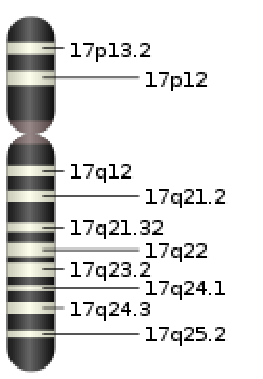
\includegraphics[height=5.7 cm]{figures/nchr17}
\end{figure}
\end{columns}
\end{frame}


\begin{frame}{Multiple Resolutions: Chromosome-17}
\begin{figure}
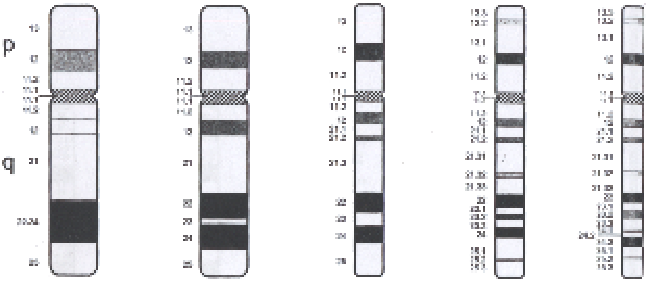
\includegraphics{figures/bands17}
\caption{G-banding patterns for normal human chromosomes at five different levels of resolution. Source: (Shaffer et. al. 2009). Example case in Chromosome:17.}
\end{figure}
\end{frame}


\begin{frame}{Multiple Resolutions: Part of Chromosome-17}
\begin{figure}
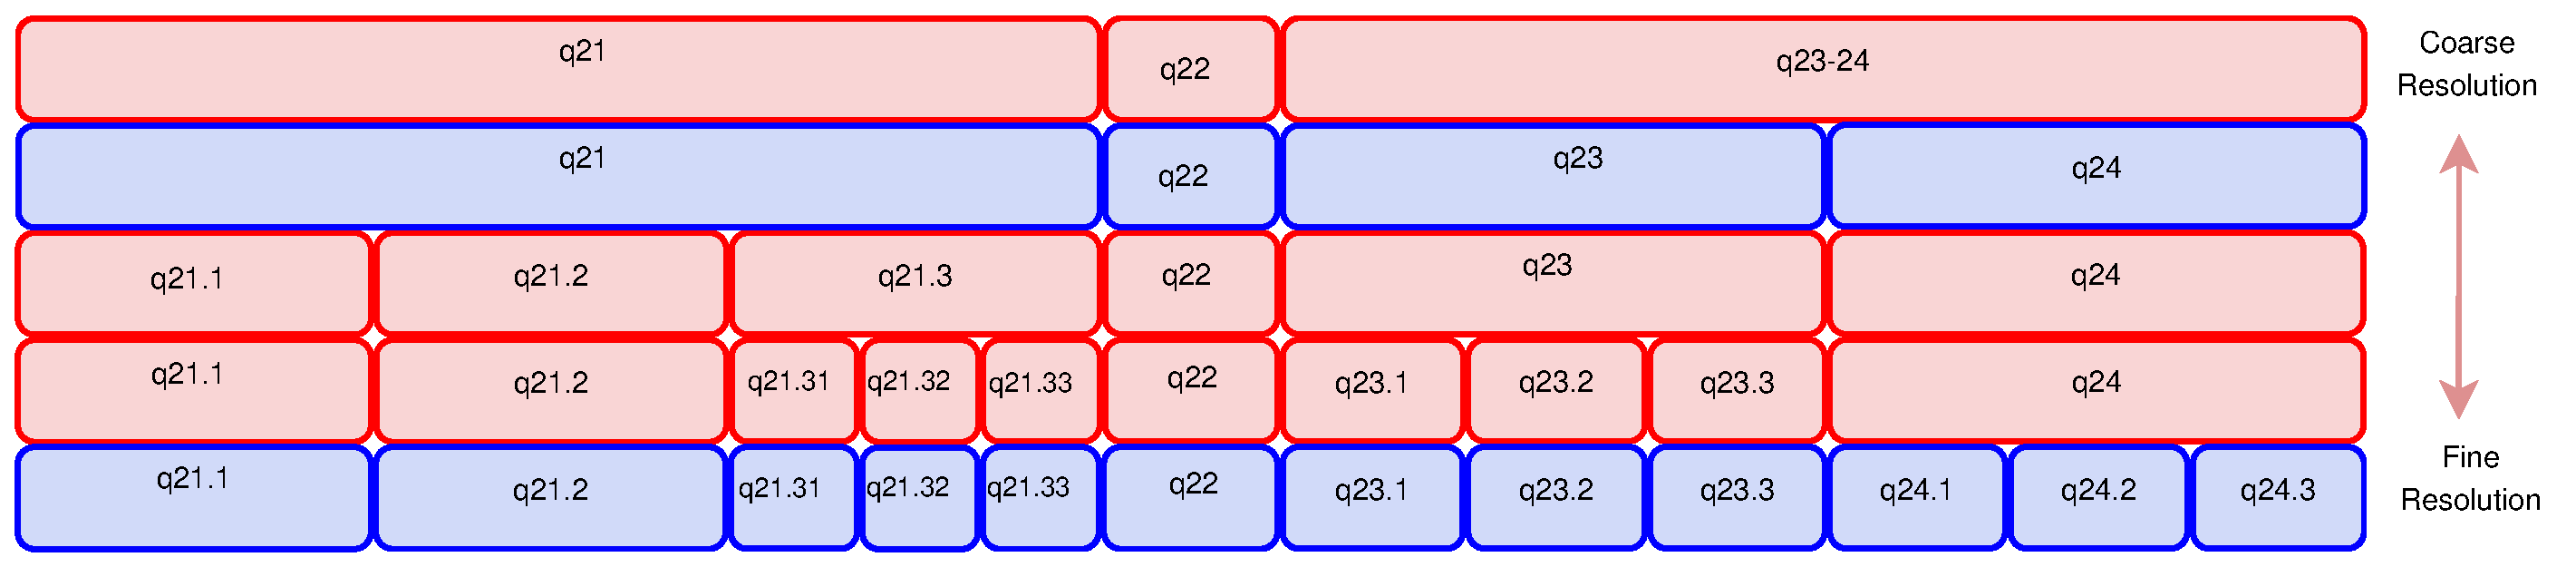
\includegraphics [scale = 0.24]{figures/mulres}
\caption{Part of chromosome 17 showing the differences in multiple resolutions.}
\end{figure}
\end{frame}


\begin{frame}{Multiple Resolutions: the problem}
\begin {alertblock}{Problem}
 Two different datasets are available in two different resolutions. How do you map into other resolutions such that patterns are preserved?  
\end {alertblock}
\end{frame}

\begin{frame}{DNA copy number amplification Dataset}
\begin{figure}[h!]
  \centering
  \subfigure [Resolution: 400] {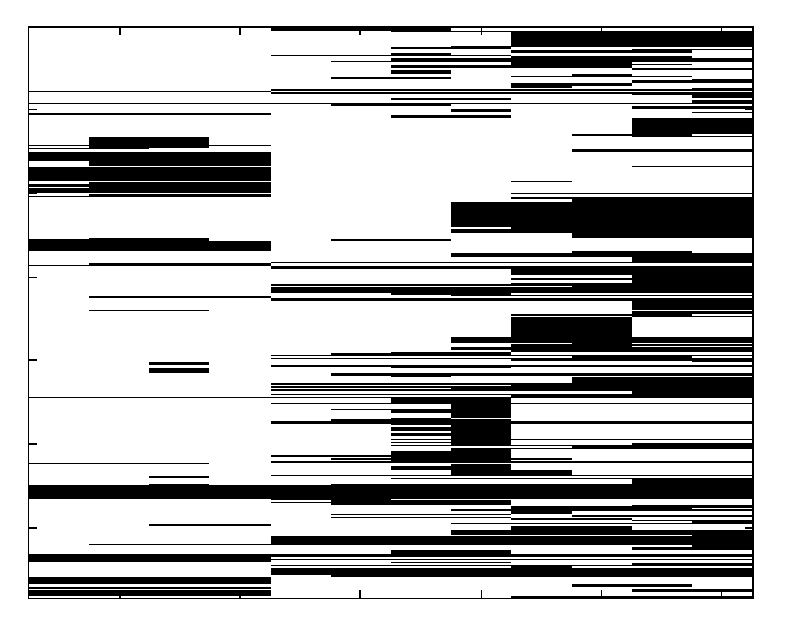
\includegraphics[scale=0.3]{figures/data}}
  \subfigure [Resolution: 850] {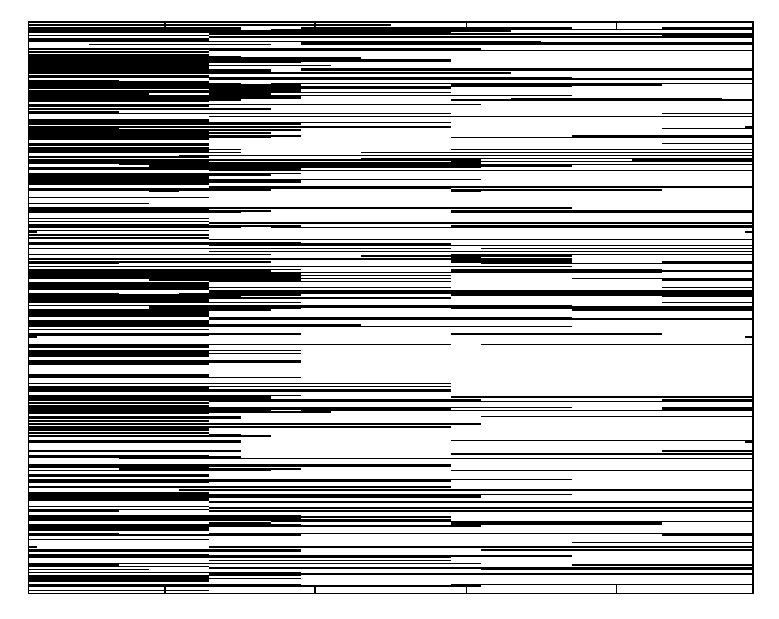
\includegraphics[scale=0.3]{figures/data850}}
  \caption{Collected by bibliomics survey of 838 journal articles during 1992-2002 in (S. Myllykangas et. al. 2006 and 2008). 4590 samples in resolution 400(left panel) and different dataset in resolution 850(Right Panel). Sparse and spatially dependent matrix. Available from the authors.}
  \label{Fig:converge}
\end{figure}
\end {frame}


\section[Sampling Resolutions]{Sampling data between different resolutions}

\begin{frame}
 \frametitle {Changing between different resolutions}
 \begin{block}{Upsampling}
 \begin{itemize}
 \item Upsampling is the process of changing the representation of data to the higher or finer resolution.
 \item Simple transformation table involving chromosome bands was used to upsample data from the resolution 400 to different finer resolutions.
 \item The transformation table were chromosome specific and resolution specific (88 tables for 5 resolutions).
 \end{itemize}
 \end{block}

\begin{table}[h!]
  \centering
  \begin{tabular}{|p{2.7cm}|p{2.7cm}|p{2.7cm}|}
    \hline
    \textbf{Resolution:400} & \textbf{Resolution:850}  \\
    \hline
    17p13	& 17p13.3 \\ \hline
    ...		& 17p13.2 \\ \hline
    ...		& 17p13.1 \\ \hline
    \end{tabular} 
\end{table}
\end{frame}


\begin{frame}
 \frametitle{Downsampling to different resolutions}
Downsampling is the process of changing the representation of the data to the lower or coarser resolution.
 \begin{block}{Complexity}
  How to map the $|0|0|1|$ or $|1|0|1|$ to $|0|$ or $|1|$
 \end{block}

\begin{enumerate}
  \item Majority Decision Downsampling
  \item OR-function Downsampling
  \item Weighted Downsampling
 \end{enumerate}
\end{frame}

\begin{frame}
\frametitle{Majority Decision Downsampling method}
\begin{figure}
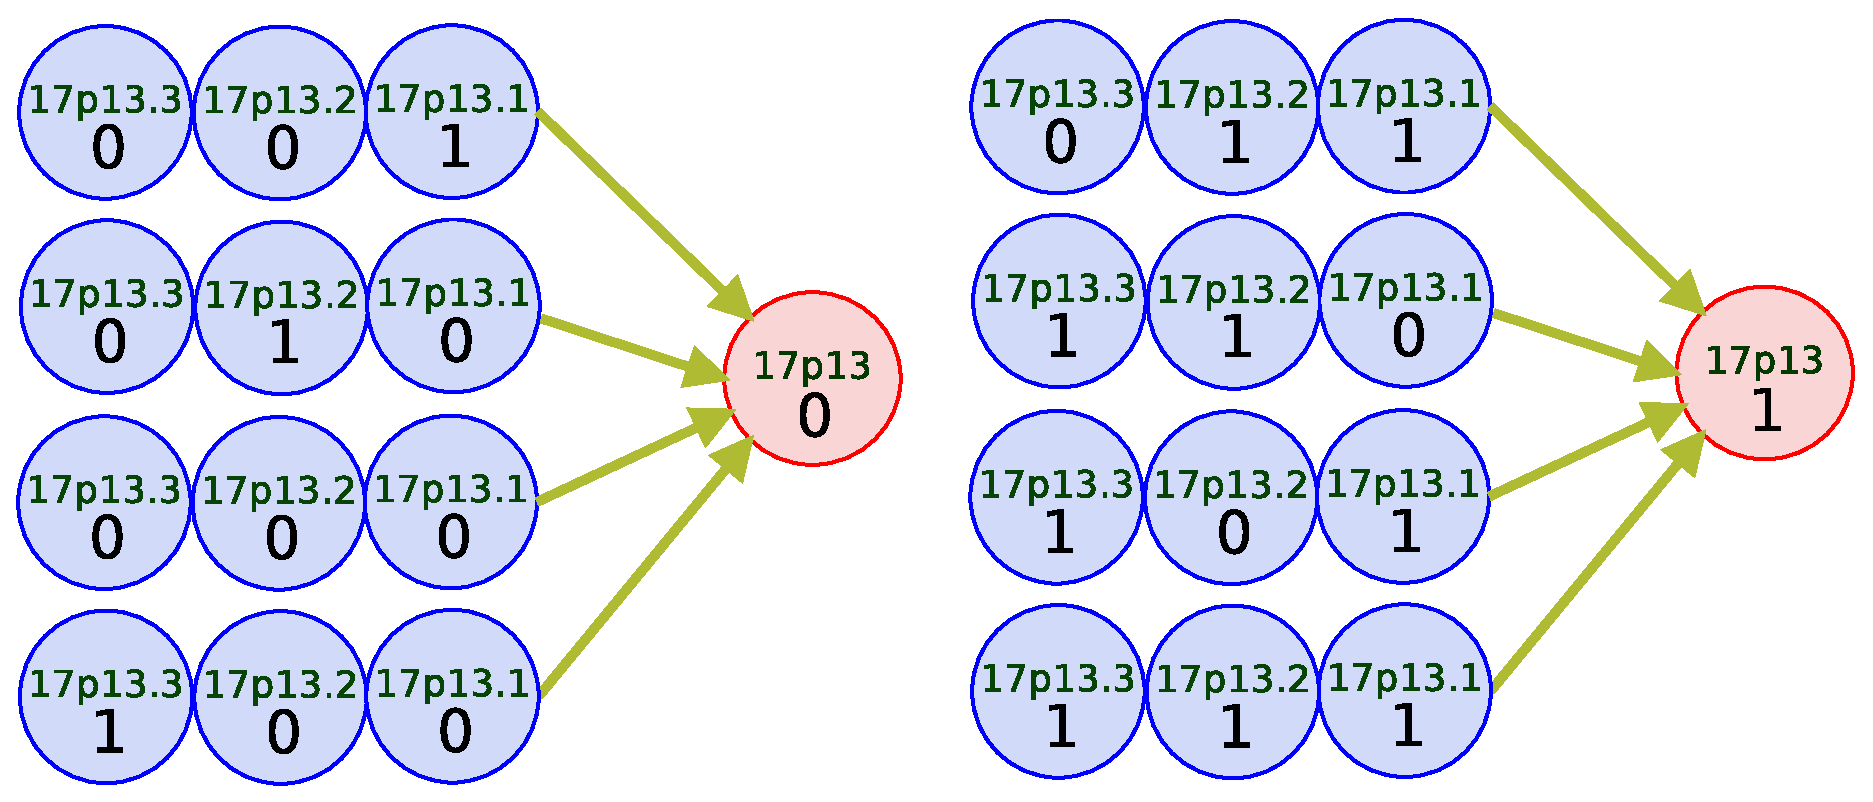
\includegraphics[scale=0.3]{figures/mdmapping}
\caption{Band in lower resolution is amplified if the majority of the bands in higher resolution is amplified. In case of a tie amplification of nearest bands are taken into consideration using ``\textcolor{blue}{golden goal}'' strategy until certain number of predefined steps.}
\end{figure}
\end{frame}

\begin{frame}
\frametitle{OR-function Downsampling Method}
\begin{figure}
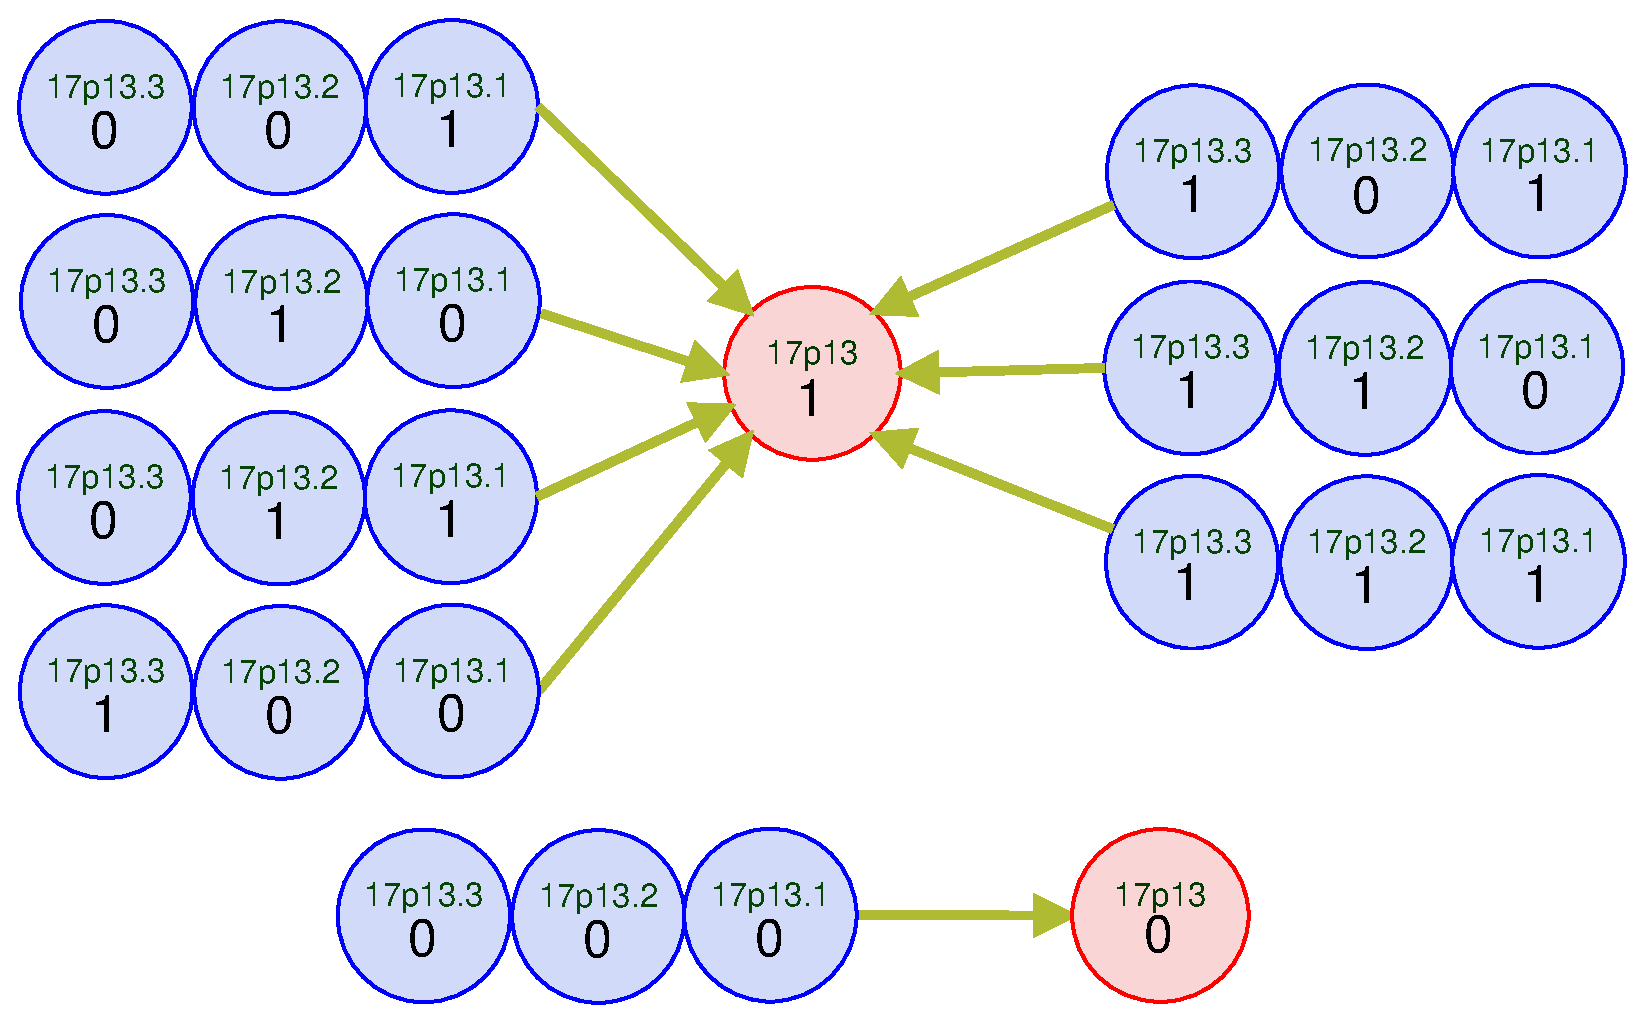
\includegraphics[scale=0.3]{figures/ptmapping}
\caption{Band in lower resolution is amplified if any of the band in higher resolution is amplified.}
\end{figure}
\end{frame}

\begin{frame}
\frametitle{Length Weighted Downsampling Method}
\begin{figure}
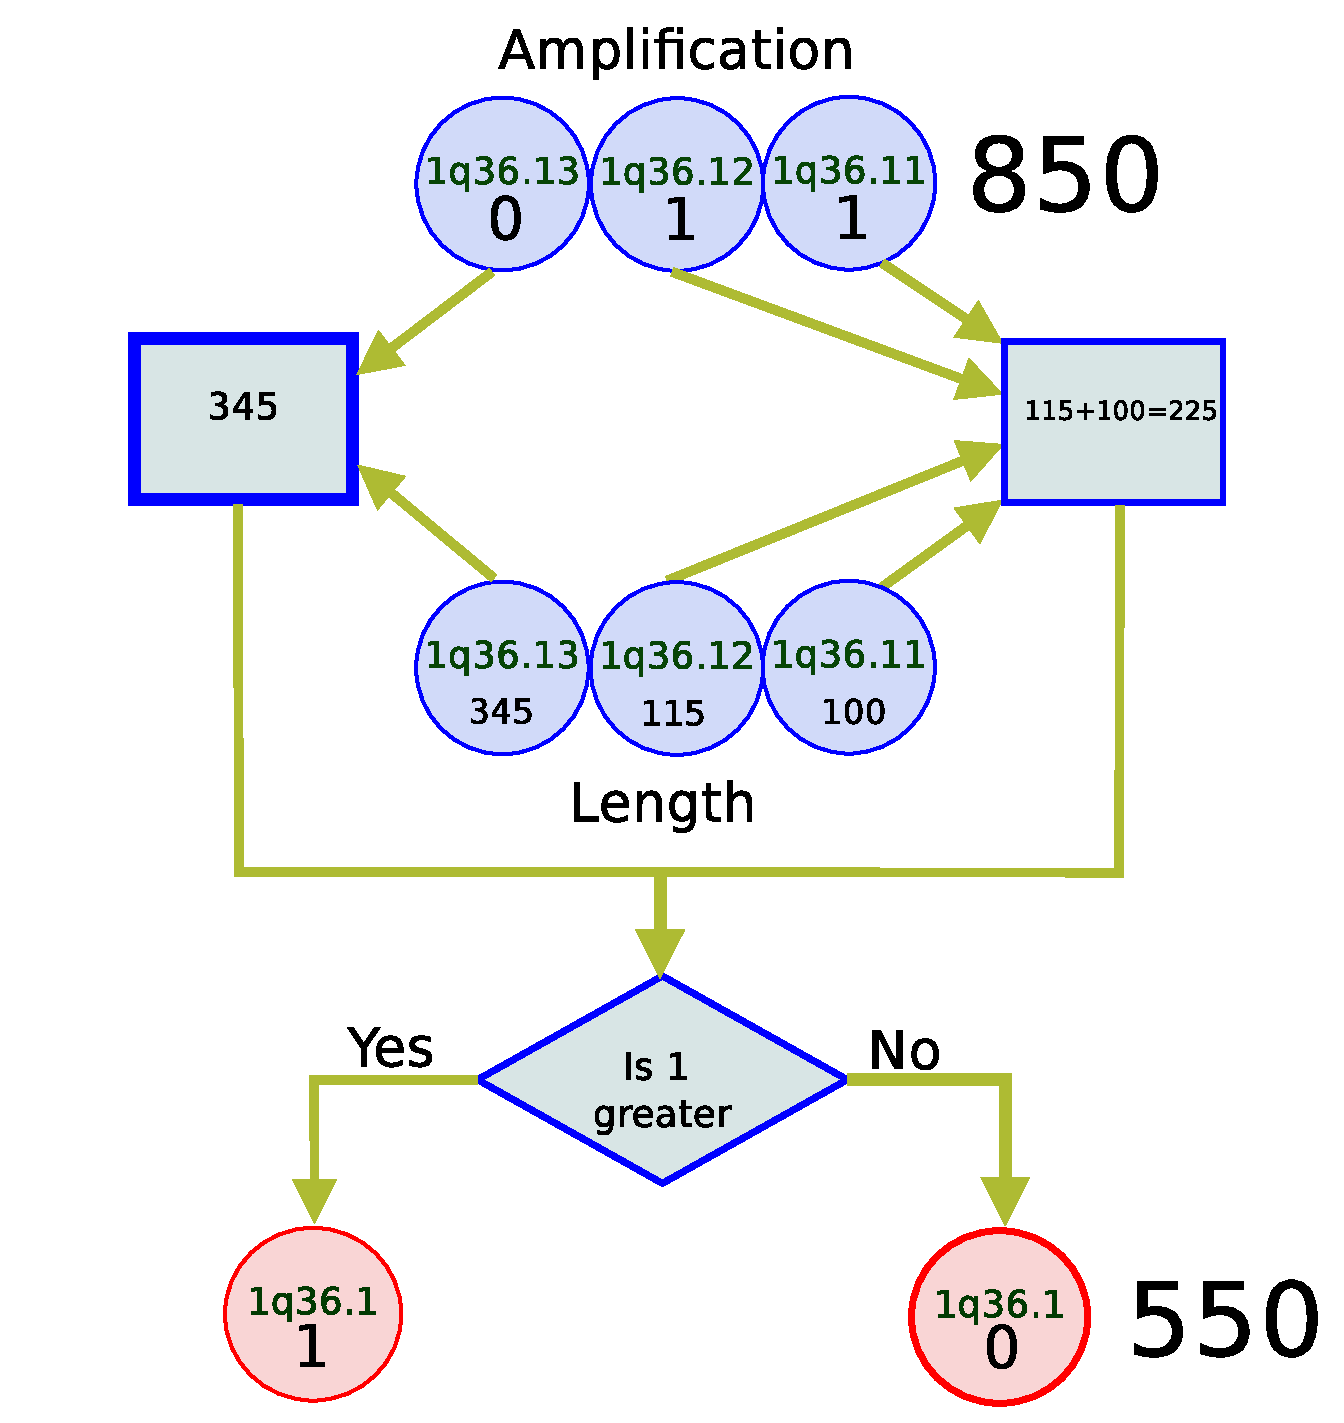
\includegraphics[scale=0.2]{figures/weighted}
\caption{Length of the bands are considered in this case. Band in lower resolution is amplified if the length of amplified band is greater.}
\end{figure}
\end{frame}

\section[Comparison]{Comparison of Different Downsampling methods}
\begin{frame}
\frametitle{Comparison of Downsampling Methods}
\begin{figure}
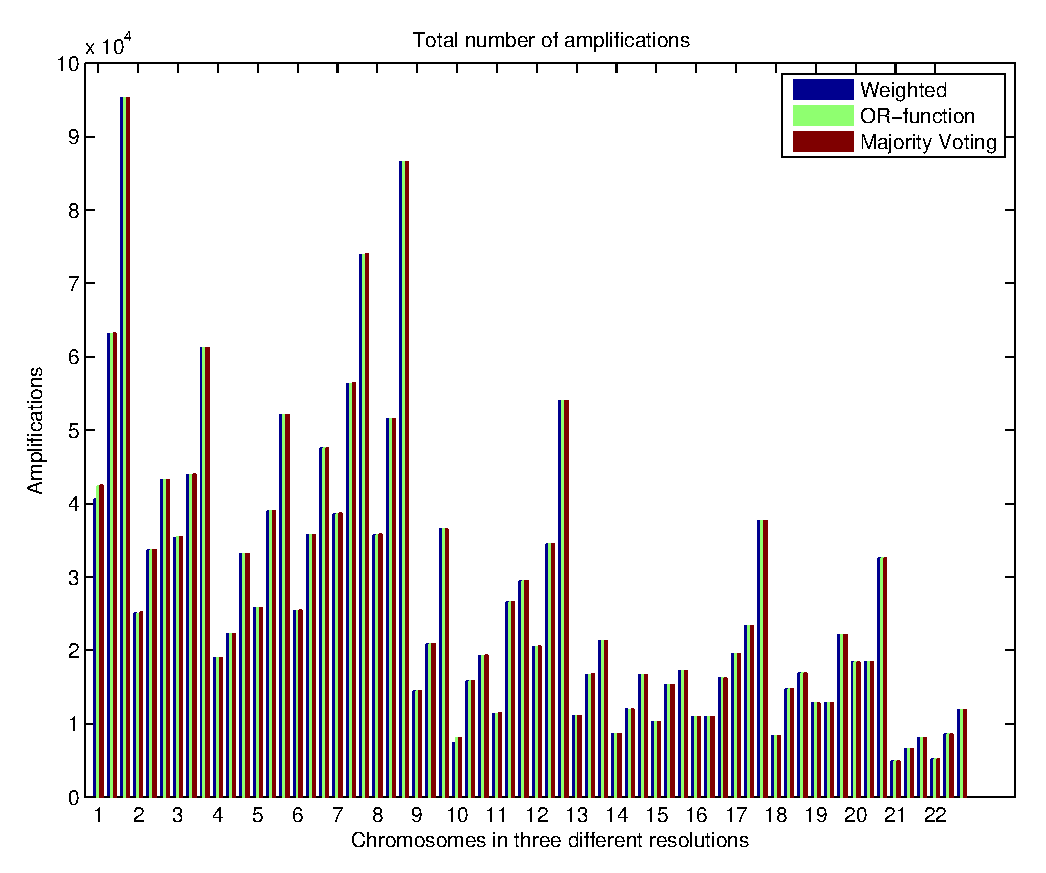
\includegraphics[height=5.3 cm]{figures/totalamp}
\caption{Total number of amplifications produced by three different downsampling methods}
\end{figure}
\end{frame}

\begin{frame}
\frametitle{Comparison of Downsampling Methods}
\begin{figure}
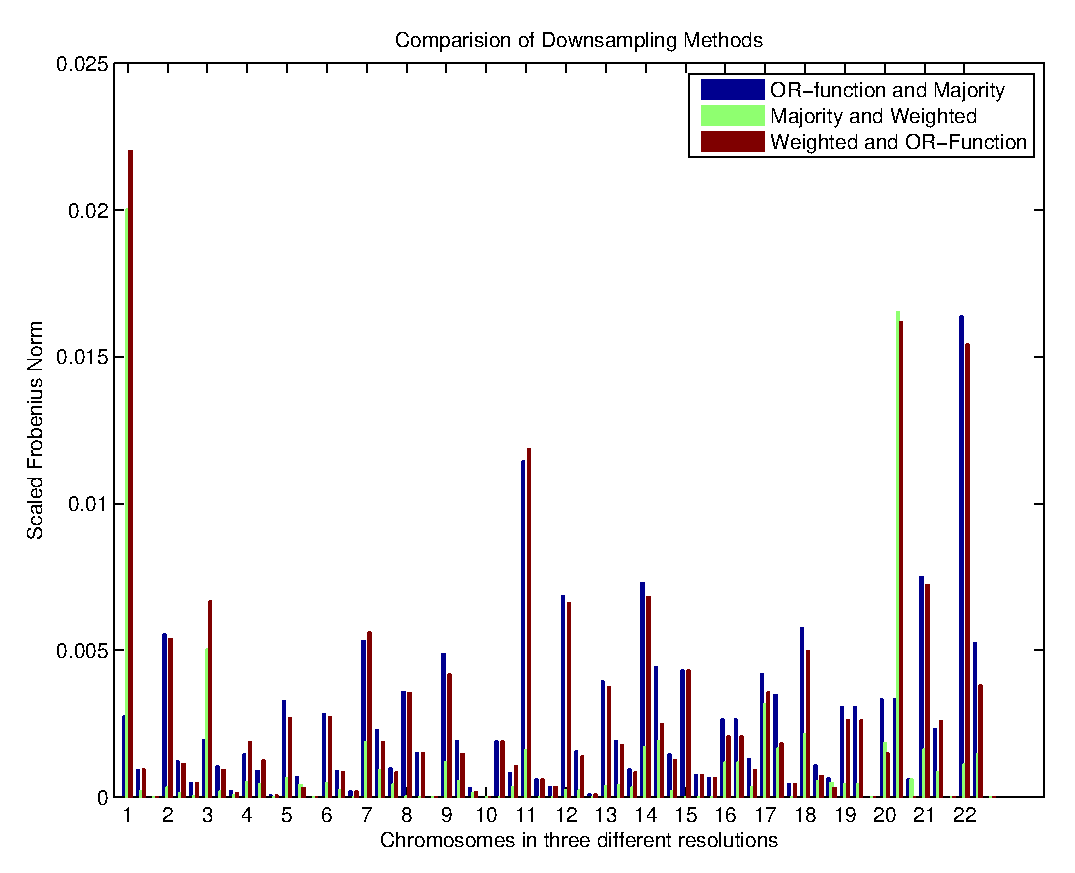
\includegraphics[height=5.3 cm]{figures/frobenius}
\caption{Comparison of three different downsampling methods : The difference measure used is scaled Forbenius norm.}
\end{figure}
\end{frame}

\section[Mixture Model]{Mixture Models of Amplification Patterns in Cancer}
\begin{frame}  \frametitle{Mixture Modelling of Cancer} 
\begin{itemize}
    \item Cancer is a collection of heterogeneous diseases     
    \item Finite Mixture Modelling of Multivariate Bernoulli Distribution \\  
    \vspace{0.1cm}  
\textcolor{blue} { $ P(x) = \sum _{j=1}^{J} \pi _{j} P(x|\theta _{j}) = \sum _{j=1}^{J} \pi _{j} \prod _{i=1}^{d} \theta_{ji}^{x_i}(1-\theta _{ji})^{1-x_{i}}$ } \\
      \vspace{0.1cm}    
     \item EM algorithm to train the Mixture Models using BernoulliMix   
\end{itemize}
\end{frame}

\begin{frame}[fragile]
  \frametitle{Model Selection: \# of Components}
\begin{figure}
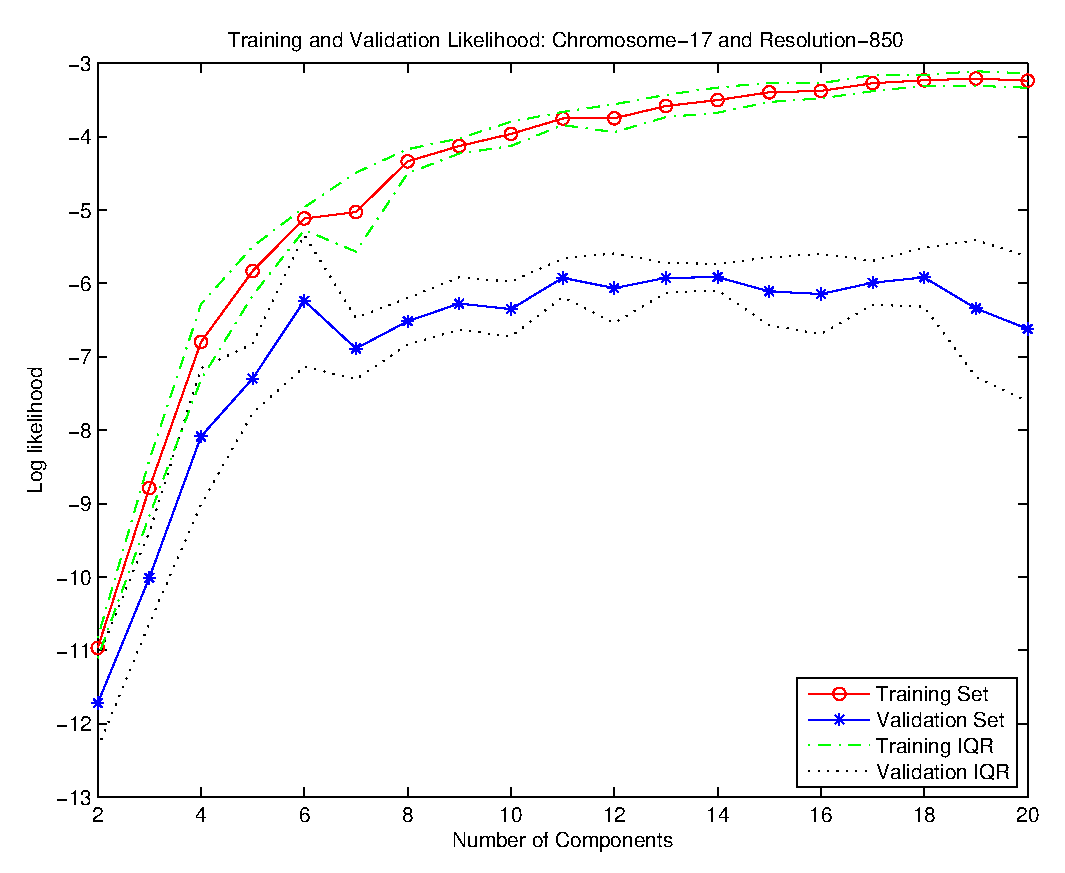
\includegraphics[scale=0.3]{figures/chr17dm850}
\caption{10-fold Cross-Validation repeated 50 times and $J$ varied between 2-20. Example case: Chromosome: 17 resolution : 850. Similar approach to (J. Tikka et. al, 2007) and (J. Hollm\'en, 2007).}
\end{figure}
\end{frame}

\begin{frame}
\frametitle{Visualization of Mixture Model}
\begin{figure}

\includegraphics[scale =2.5]{figures/modelvis}
\caption{A visualization of one of the final model trained for chromosome-17 in resolution: 850.}
\end{figure}
\end{frame}

\begin{frame}
\frametitle{Results of Mixture Models}
\begin{table}[h!]
  \centering
  \begin{tabular}{|l|c|c|}
    \hline
    \textbf{Data Resolution} & \textbf{J} &\textbf{Likelihood}  \\
    \hline
    Original in 393	&	8	& 	-3.39  \\ \hline
    Original in 850	&	8	& 	-4.75 \\ \hline
    Downsampled to 393	&	6	& 	-3.41  \\ \hline
    Upsampled to 850	&	6	& 	-5.23  \\ \hline
    Combined  in 393	&	7	& 	-3.36  \\ \hline
    Combined in 850	&	7	& 	-5.11  \\ \hline     
  \end{tabular}
  \caption{Results of experiments on chromosome-17. J denotes the selected number of component distributions. }\label{Tab:results}
\end{table}
\end{frame}

\section[MFI]{Maximal Frequent Itemset}
\begin{frame}{Are Maximal Frequent Itemset Preserved?}

\begin{table}[h!]
  \centering
  \begin{tabular}{|c c p{4cm}|}
    \hline
    \textbf{Resolution 400} &   &\textbf{Resolution 850}  \\
    \hline
   Frequent Itemset	&	$\Rightarrow$	& \hspace{0.2cm} Frequent Itemset  \\ 
    \{6,7,8\}	&	$\Rightarrow$	&\{8,9,10,11,12,13,14\}  \\ 
    $\Updownarrow $ 	&		& \hspace{1.5cm}$\Updownarrow $ \\ 
    Chromosome Bands	&	$\Rightarrow$	& \hspace{0.15cm} Chromosomse Bands  \\ 
   \{17q11.2, 17q12, 17q21\} &	$\Rightarrow$	& \{17q11.2, 17q12, 17q21.1, 17q21.2, 17q21.31, 17q21.32, 17q21.33 \}  \\ \hline
    
  \end{tabular}
  %\caption{Results of experiments on chromosome-17. J denotes the selected number of component distributions. }\label{Tab:results}
\end{table}
\end{frame}

%\textbf{Resolution:400} $\Leftrightarrow$ \textbf{Resolution:850}
%MFI:\{5,6,7\} \Rightarrow MFI: \{7,8,9\} 
%\Updownarrow                          \Updownarrow 
%Bands: \{17q11.1, 17q11.2, 17q12 \} \Rightarrow Bands: \{17q11.1, 17q11.2, 17q12 \}
%MFI:\{6,7,8\} $\Rightarrow$ MFI: \{8,9,10,11,12,13,14\} 
%$\Updownarrow $                         $\Updownarrow $
%Bands: \{17q11.2, 17q12, 17q21\} $\Rightarrow$ Bands: \{17q11.2, 17q12, 17q21.1, 17q21.2, 17q21.31, 17q21.32, 17q21.33 \}
%\end{frame}


\section{Summary and Conclusions}
\begin{frame}
 \frametitle{Something to take home about}
 \begin{itemize}
      \item Downsampling and upsampling to work with various resolutions of data useful for database integration
      \item Mixture models of 0-1 data in different resolutions
      \item Effect of Resolution and Sample Size on likelihood and number of components
 \end{itemize}
\end{frame}
\end{document} 